\chapter{Technológiai háttér} \label{technologyChapter}
Ebben a fejezetben szeretném ismertetni a GPU porgramozáshoz felhasznált szoftver- és hardveregyüttest. Először a grafikus segédprocesszoron történő általános célú programozást tárgyalom, majd bemutatom az Nvidia\textsuperscript{TM} által erre kifejlesztett párhuzamos számítási platformot, a CUDA keretrendszert. Részletezem a megértéshez szükséges fontosabb fogalmakat, valamint bemutatom a CUDA platformon fejlesztéshez elengedhetetlen lépéseket. A fogalmak összegyűjtéséhez nagymértékben ihletett nyújtott többek között Király Gábor diplomamunkája, mely hasonló témakörrel foglalkozik. \cite{kvantum_optim}

\section{GPGPU}
A GPGPU (general-purpose computing on graphics processing units) egy olyan
szoftverfejlesztési gyakorlat, melynek során a grafikus feldolgozóegységet (GPU) általános
célú számítási műveletek elvégzésére használjuk. \cite{kvantum_optim} Korábban a GPU-t azért találták fel, hogy a grafikus felületek elterjedése után a renderelési, 2D-s vagy 3D-s megjelenítési feladatok terén tehermentesítse a CPU-t. Később kiderült, hogy a GPU alkalmas általánosabb megközelítésekre is, bizonyos aritmetikai utasítások kifejezetten hatékonyan tudnak működni rajta.

\subsection{Motiváció}
Az 1980-as években megjelentek az első személyi számítógépek (PC-k), melyek központi feldolgozóegységei (CPU) kezdetekben néhány MHz-es belső órajellel működtek. Akkor az volt a számítástechnikai fejlesztőmérnökök fő eszköze a számítási gyorsaság növelésére, hogy az órajelfrekvenciát növelték. Ez frekventáltabb utasítás-végrehajtást biztosított, és evidens volt, hogy a nagyobb frekvencia nagyobb számítási erővel is jár. Számos kiváló mérnöki megoldás született, ezek közül talán az egyik legjelentősebb találmány a fáziszárt hurok (Phase-Locked Loop - PLL). A PLL egy olyan Szabályozható hurok, amely (a részleteket mellőzve, nem tárgya dolgozatomnak) egy bemeneti referenciafrekvenciát tud megsokszorozni. Nélküle gyakorlatilag képtelenség lett volna felhasználói szinten 50-60 MHz fölé menni a személyi számítógépek belső órajelénél. Nagyjából 30 évvel később elérték a hardverfejlesztők, hogy a legtöbb asztali processzor órajele 1GHz és 4GHz között legyen képes működni, ez az eredeti PC-k operatív belső frekvenciájának több, mint az ezerszerese. Napjainkban változás látható a fejlesztési trendekben, ugyanis az órajelnövelést a processzorok hődisszipációja felülről korlátozza. Egyelőre nem tűnik könnyen lehetségesnek 5GHz fölé menni úgy, hogy közben az eszköz helyes működése garantálható legyen. A különböző hűtési technológiák (léghűtés, vízhűtés) bizonyos fokig tudnak javítani a sebességen, viszont nagyságrendeket ugorni velük sem lehetséges. 
A számítógépgyártók mai napig új, alternatív megoldásokat keresnek a számítási teljesítmény növelésére. Napjainkban a kutatásoknak két nagy témája van. Egyik a kvantumszámítógépek témaköre, amit dolgozatomban nem részletezek. Másik aktívan vizsgált lehetőség a párhuzamosítás minél több szálon. Már a CPU-k fejlesztésénél is megfigyelhető, hogy inkább a minél több processzormag telepítése az iparági trend.

\begin{figure}[ht!]
	\centering
	
\includegraphics[width=150mm, keepaspectratio]{figures/CPU-cores-trend.png}
	\caption{Látható, hogy kb. 2010-re befejeződött a CPU-k órajelfrekvencia-növekedése, helyette egyre nőni kezdtek a magok számai. \cite{CPUcores} }
\end{figure}

Párhuzamosításra legalkalmasabb a grafikus segédprocesszor, a GPU, hiszen felépítéséből adódóan erre készült. Amíg a CPU feladata az, hogy műveletek egy adott szekvenciáját, és annak minden utasítását a lehető leggyorsabban hajtsa végre, addig a GPU célja minél több szál (akár több ezer, vagy több tízezer) párhuzamos futtatása. A videokártyák előnye akkor válik láthatóvá, ha ugyanazt az utasítást több nagy adattömbön kell végrehajtani. Ez az úgynevezett SIMD megközelítés (Single Instruction Multiple Data). \cite{kvantum_optim}
Az \ref{TransistorsInGpu}. ábra szemlélteti, hogy a CPU-hoz képest a GPU-n arányaiban több tranzisztor van adatfeldolgozásra rendelve, cserébe a gyorsítótárazás és a folyamatvezérlés (feltételkiértékelések, ciklusszervezések) kisebb hangsúlyt kapott.

\begin{figure}[ht!]
	\centering
	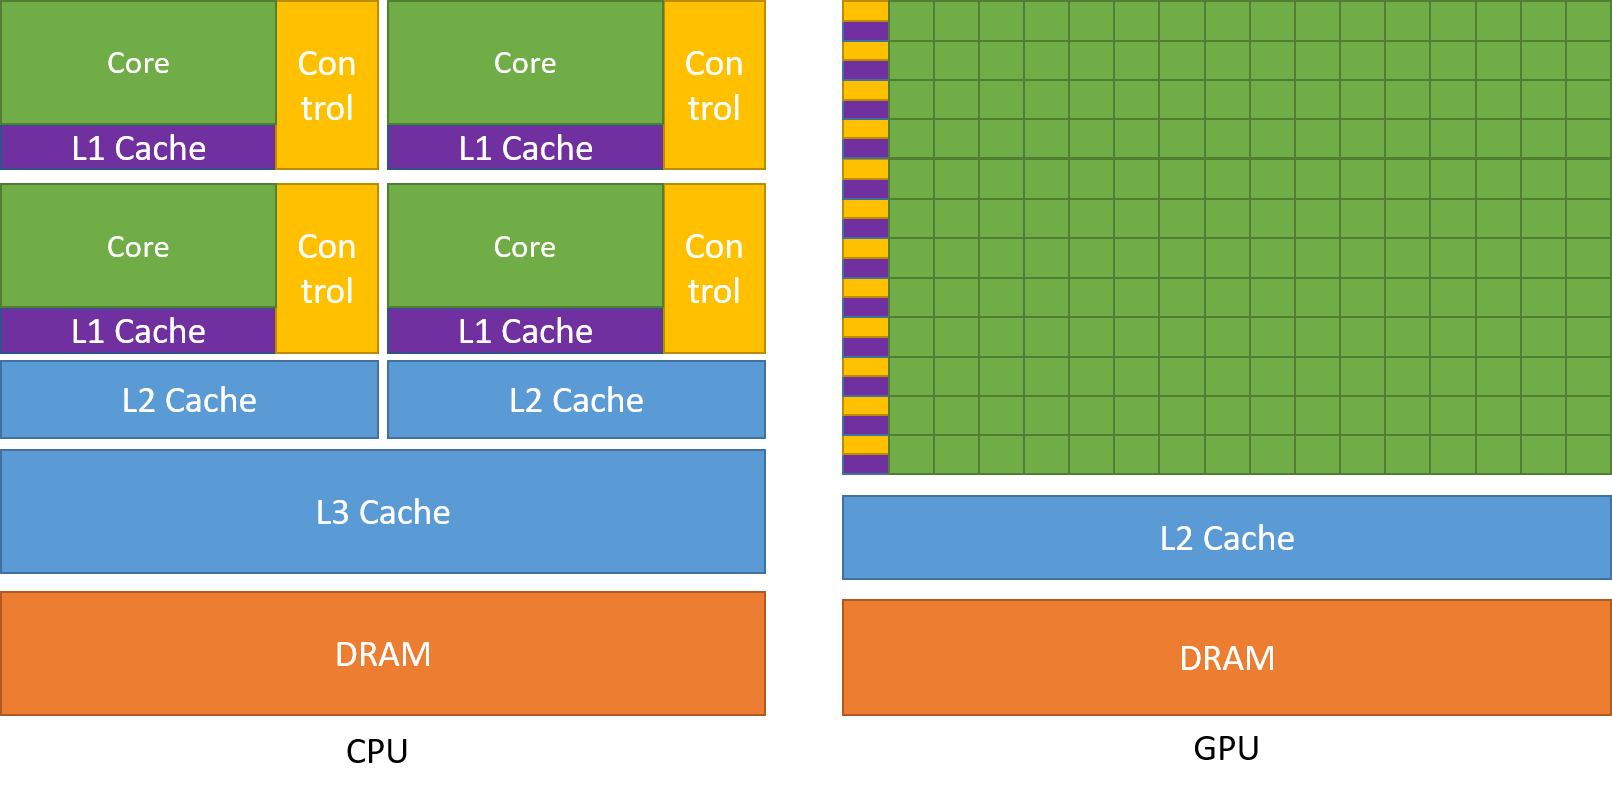
\includegraphics[width=150mm, keepaspectratio] {figures/gpu-devotes-more-transistors-to-data-processing.png}
	\caption{Látható, hogy a gyorsítótárak és a vezérlés rovására nőtt az adatfeldolgozásra szánt tranzisztorok számára. Ez alkalmas lebegőpontos műveletek nagyfokú párhuzamosítására. \cite{CUDAdoc} \label{TransistorsInGpu} }
\end{figure}


A videokártya sokkal nagyobb utasítás-áteresztőképességet, valamint memória-sávszélességet biztosít, mint a CPU hasonló ár és energiafogyasztás mellett. Egyéb számítási eszközök, mint az FPGA-k is lehetnek nagyon energiatakarékosak, viszont azok sokkal kevésbé rugalmasan programozhatóak, mint a GPU-k, ezért a fejlesztési idő sokkal hosszabb lesz és az alkalmazást nehezebb karbantartani. \cite{CUDAdoc}



\section{CUDA}
Többféle keretrendszer is megvalósítja a GPGPU szabta alapelveket. Munkám a CUDA ( Compute Unified Device Architecture ) rendszerét használtam. A CUDA egy, az NVIDIA által fejlesztett párhuzamos számítási platform és API (felhasználói interfész), amely szoftveres támogatást nyújt az ezzel kompatibilis grafikus feldolgozóegységek általános célú programozására \cite{kvantum_optim}. 

A programozás C vagy C++ nyelven történhet, melyet minimális nyelvi kiegészítésekkel bővítettek, többek között a szálkezelés rendszerszintű használata érdekében. A CUDA programozás tanulásához elérhető egy felettébb kiterjedt dokumentáció a gyártó weboldalán, melyet folyamatosan frissítenek. \cite{CUDAdoc}

\subsection{Programozási modell }
A továbbiakban összefoglalom a legfontosabb fogalmakat úgy, hogy ismertetem, azok hogyan lettek megvalósítva C++ programozási nyelven.

\subsubsection{Kernel, és a többi függvénytípus}
A programozó speciális függvényeket definiálhat, melyeket kernelnek nevezünk. A kernel létesít kapcsolatot a CPU (host) és GPU (device) között. A CPU hívja meg a függvényt, amit aztán a GPU hajt végre, tehát a kernelfüggvény törzse a videokártyán fut végig. Minden egyes kernel példányt egy számára megadott szál hajt végre.
A kernel a "\textit{\_\_global\_\_}" kulcsszóval definiálható. Ezt a függvény fejléce elé kell írni, ekkor tudja tudni a szoftverkörnyezet fordítóprogramja, a compiler, hogy mostantól GPU kódként kell értelmezze a programot. 

Egyéb kulcsszavak is léteznek. Egyik a "\textit{\_\_host\_\_}", ami azt jelzi, hogy CPU által hívott, majd ugyanúgy általa futtatandó kódrészlet következik. Ha nem adunk meg egy függvény elé kulcsszót, akkor azt a preprocesszor host függvénnyé írta át, tiszta CPU kódként értelmezi, mintha nem is lenne a szoftverkörnyezet mögött a CUDA platform. Másik használható jelző a "\textit{\_\_device\_\_}", amely tisztán GPU függvényt jelez. A két kulcsszó vegyíthető: amennyiben azt írjuk, hogy "\textit{\_\_device\_\_ \_\_host\_\_}", a fordító ezt minden egyes híváskor a végrehajtó saját kódjának tekinti, vagyis nem hajt végre vezérlésátadást az eszközök között. Hasznosítható például függvénykönyvtárak GPU-ra kiterjesztésére.

\paragraph{}
Az, hogy a kernelt egy adott híváskor hány CUDA szálon szeretnénk futtatni, az új nyelvi elemként megjelenő <<< · · · >>> végrehajtási konfiguráció szintaxissal tudjuk specifikálni. Sajnos a Visual Studio még szintaxishibaként kezeli \textcolor{red}{verziószám?}, ezért a programozónak érdemes odafigyelni, hogy milyen IntelliSense hibaüzeneket vesz figyelembe. A \ref{invalidErrors}. ábrán például olyan fogalmakra jelez a fejlesztői környezet, amelyek a keretrendszer adta bővítményekben vannak definiálva. Minden, a kernelt végrehajtó szál egy egyedi thread azonosítót kap, mely a beépített threadIdx változón keresztül érhető el a kernelből.

%TODO verziószám

\begin{figure}[ht!]
	\centering
	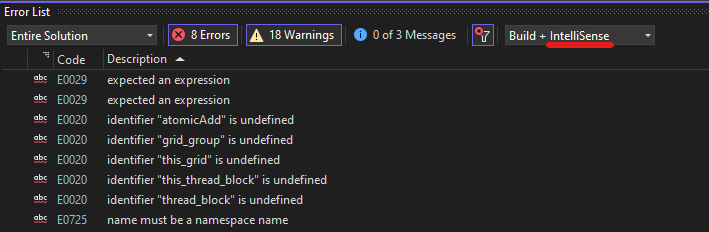
\includegraphics[width=150mm, keepaspectratio] {figures/invalidIntellisenseErrorMessages.png}
	\caption{Bizonyos hibaüzeneteket azért kaphatunk, mert a Visual Studio által használt Intellisense nem ismeri a CUDA által tett kiegészítéseket. Ezeket figyelmen kívül lehet hagyni \label{invalidErrors} }
\end{figure}

\paragraph{Példa:} A hivatalos dokumentáció az alábbi példát adja kernel definícióra. A kódrészlet az N méretű A és B vektorok összeadását végzi és az eredményt a C vektorban tárolja:

\begin{lstlisting}[style=CStyle]
	#define N 1024
	
	// Kernel definition
	__global__ void VecAdd(float* A, float* B, float* C)
	{
		int i = threadIdx.x;
		C[i] = A[i] + B[i];
	}
	
	int main()
	{
		...
		// Kernel invocation with N threads
		VecAdd<<<1, N>>>(A, B, C);
		...
	}
\end{lstlisting}

Megfelelő CPU programkörnyezet hozzáadásával ellenőrizhető, hogy a példában adott kernel tényleg helyes eredményt ad.

\subsubsection{Szálkezelés}
Ahhoz, hogy CUDA programunk megfelelően működjön, a szálainkat rendszereznünk kell. 

Most bemutatom, hogy CUDA API-ban milyen típusú szálak léteznek, és ezeket hogyan lehet különböző szintű szinkronizációkba hozni. Ezen fejezetrészhez intenzíven tanulmányoztam az NVIDIA hivatalos fórumának bejegyzéseit, amit mivel az ott dolgozó fejlesztőmérnökök szerkesztenek, relevánsnak tekintettem. Az egyik leghasznosabb cikket a "Cooperative Groups" nevű bővítményről találtam \cite{CUDAcoopgroups}.

Hatékony párhuzamosított programnak három alappillére van: \cite{kvantum_optim}
\begin{enumerate}
	\item \emph{Szálak csoportosításának hierarchiája}: MultiGrid - Grid - Blokk - Szál
	\item \emph{A szálak között megosztott memória: shared memory}
	\item \emph{A szálak közti szinkronizáció}
\end{enumerate}
Foglalkozzunk jelen esetben a 3. ponttal, a szinkronizálással. Szinkronizáció szükséges ahhoz, hogy elosztott programunk biztonságos, fenntartható és moduláris legyen. A CUDA 9 bevezette az ún. \textbf{Kooperatív csoport} nevű absztrakciót (angolul Cooperative Groups) \cite{CUDAdoc_coopGroups}, amely erős támogatást nyújt a kerneleknek ahhoz, hogy dinamikusan alakíthassanak ki csoportokat a szálak között.

\paragraph{}
Korábban a CUDA API egy nagyon egyszerű, de csak speciális esetekben működő megoldást biztosított a szinkronizáció kérdésére, a blokkon belüli "barrier" szinkronizációt: A "\_\_syncthreads()" függvény addig nem engedte tovább futni a szálakat, amíg \textbf{a blokkon belül} minden még futó szál el nem jutott az adott pontig. Belátható, hogy nagy szál szám mellett ez nem elég, ugyanis egy blokkon belül jelenlegi GPU-kon legfeljebb 1024 szál futhat. Ha mi több, mint 1024 threadből álló programot írnánk, azaz több Streaming multiprocessor (SM) futna egymással párhuzamosan, akkor ezek összehangolását eddig nem tudtuk volna megfelelő szoftveres támogatással elvégezni. Másik probléma az, hogyha a szálainknak csak egy kis, adott számú (például 4 vagy 32, de tipikusan 2-hatvány) részhalmazát akarjuk összehangolni akkor korábban azt sem tudtuk szépen megoldani.

\paragraph{}
Leegyszerűsítve a Cooperative Groups egy API Support Package, ami szálak csoportosítását és szinkronizálását segíti CUDA programokban. A Package nagy része az összes CUDA 9-el kompatibilis GPU-ra működik, azaz Kepler és későbbi architektúrákkal (Compute Capability 3.0+) kompatibilis.

Ahhoz, hogy élhessünk a csomag nyújtotta lehetőségekkel, be kell illeszteni az alábbi headert .cu vagy .cuh kiterjesztésű fájlunk fejlécébe.

\begin{lstlisting}[style=CStyle]
	#include <cooperative_groups.h>
\end{lstlisting}

A típusok és interfészek a "cooperative\_groups" C++ névtérben vannak definiálva, így mindig prefixként ki kell írjuk, hogy "cooperative\_groups::", vagy betöltjük a névteret a "using" direktívával. Én a munkám során a "using" megoldást választottam.

\begin{lstlisting}[style=CStyle]
	using namespace cooperative_groups; // Névtér betöltése
	using cooperative_groups::thread_group; // stb. 
	namespace cg = cooperative_groups; // Használhatunk rövid aliast is
\end{lstlisting}

\paragraph{Thread csoportok}
Az egyik legfontosabb típus a csomagon belül a "thread\_group" típus, ami threadek, azaz szálak csoportját tudja kezelni. Ezt örökölteti le az összes, később tárgyalandó csoport objektum. Alapvető függvények rájuk:

- Megkaphatjuk a csoport méretét, azaz a benne futó szálak számát a size() metódussal. Használható túlcímzés elleni védelemre
\begin{lstlisting}[style=CStyle]
	unsigned size();
\end{lstlisting}
- Megkaphatjuk a hívó thread indexét (0 és size()-1 közötti) a thread\_rank() metódussal
\begin{lstlisting}[style=CStyle]
	unsigned thread_rank();
\end{lstlisting}
- Megvizsgálhatjuk a csoport érvényességét az is\_valid() függvénnyel
\begin{lstlisting}[style=CStyle]
	bool is_valid();
\end{lstlisting}


\paragraph{Thread csoportokon végrahajtható kollektív (egyenhatású) műveletek} -
A thread csoportok megadják a lehetőséget, hogy együttesen hajtsunk rajtuk végre műveleteket. Legegyszerűbb operációink egyike a szinkronizálás, ami annyit tesz, hogy a csoport tagjait nem engedi túl egy műveletsoron addig, míg minden tagja el nem jut az adott pontig. Az összes thread csoport fajta támogatja a szinkronizálást, azonban mindegyik kicsit másképp.

Egy adott g csoporthoz tartozó szálakat a kollektív sync() metódussal, vagy g-re a cooperative\_groups::synchronize() függvényt meghívva szinkronizálhatjuk. Ezek a már korábban emlegetett barrier szinkronizációt hajtják végre.
\begin{lstlisting}[style=CStyle]
	g.sync();           // g szinkronizálása
	cg::synchronize(g); // ekvivalens megoldás
\end{lstlisting}

\hypertarget{reducesum}{A következő egyszerű példában egy device (GPU-n futtatott) függvény} szerepel kooperatív csoportok felhasználásával. Amikor egy thread csoport meghívja, a szálak kiszámolják a szálanként kapott értékek összegét a csoporton belül.
\begin{lstlisting}[style=CStyle]
	using namespace cooperative_groups;
	__device__ int reduce_sum(thread_group g, int *temp, int val)
	{
		int lane = g.thread_rank();
		
		// Each iteration halves the number of active threads
		// Each thread adds its partial sum[i] to sum[lane+i]
		for (int i = g.size() / 2; i > 0; i /= 2)
		{
			temp[lane] = val;
			g.sync(); // wait for all threads to store
			if(lane<i) val += temp[lane + i];
			g.sync(); // wait for all threads to load
		}
		return val; // note: only thread 0 will return full sum
	}
\end{lstlisting}

\paragraph{Thread Blokk}
Az első thread csoport fajta a Thread blokk. A Cooperative Groups azért vezette be ezt az adattípust, hogy explicit reprezentálja a CUDA programozás azonos nevű, egyik fontos fogalmát. A szálak egy-, kettő-, vagy háromdimenziós logikai egységbe szervezhetők, amit \textbf{blokk}nak nevezünk. Ez a megoldás egy természetes módot nyújt arra, hogy vektorok vagy mátrixok elemein hajtsunk végre számításokat. 
Az egy blokkba tartozó szálak számát havdveres megfontolások felülről korlátozzák: mivel ezeknek a threadeknek közös processzormagon kell futniuk és a mag korlátos memória-erőforrásain kell osztozniuk, nem fogalhatnak el túl nagy helyet. A jelenlegi GPU-k egy blokkban legfeljebb 1024 thread futtatását támogatják, viszont a kernel több egyenlő méretű blokkban futtatható, ezért a szálak száma egyenlő a blokkonkénti szálak száma és a blokkszám szorzatával. \cite{kvantum_optim}
Egy thread blokk példánya az alábbi módon inicializálható:
\begin{lstlisting}[style=CStyle]
	thread_block block = this_thread_block();
\end{lstlisting}

Azon threadek, amelyek ugyanazon beépített CUDA blockIdx értékkel rendelkeznek, ugyanazon thread blokkba tartoznak. A blokkok szinkronizálása nagyon hasonló a korábban emített \_\_syncthreads() metódushoz. A következő kódok mind ugyanolyan hatást érnek el: (feltéve, ha a thread blokk összes szála elér odáig)
\begin{lstlisting}[style=CStyle]
	__syncthreads();
	block.sync();
	cg::synchronize(block);
	this_thread_block().sync();
	cg::synchronize(this_thread_block());
\end{lstlisting}

A "thread\_block" adattípus kiterjeszti a "thread\_group" interfészt két, blokk-specifikus tagfüggvénnyel. Ezek megfeleltethetőek a CUDA API blockIdx és threadIdx tagváltozóinak.
\begin{lstlisting}[style=CStyle]
	dim3 group_index();  // 3-dimenziós blokk index griden belül
	dim3 thread_index(); // 3-dimenziós thread index blokkon belül
\end{lstlisting}

Az alábbi egy egyszerű kernel, ami a korábban látott \hyperlink{reducesum}{"reduce\_sum()"} device függvényt használja egy tömb elemeinek összegzésére. Gyorsítás érdekében több, párhuzamosan elvégzett rész összeadással kezd (thread\_sum()). A kernel thread blokkokat használ az összegzésre, és az atomikus "atomicAdd()" metódussal adja össze a részösszegeket.

\begin{lstlisting}[style=CStyle]
	__device__ int thread_sum(int *input, int n) 
	{
		int sum = 0;
		
		for(int i = blockIdx.x * blockDim.x + threadIdx.x;
		i < n / 4; 
		i += blockDim.x * gridDim.x)
		{
			int4 in = ((int4*)input)[i];
			sum += in.x + in.y + in.z + in.w;
		}
		return sum;
	}
	
	__global__ void sum_kernel_block(int *sum, int *input, int n)
	{
		int my_sum = thread_sum(input, n);
		
		extern __shared__ int temp[];
		auto g = this_thread_block();
		int block_sum = reduce_sum(g, temp, my_sum);
		
		if (g.thread_rank() == 0) atomicAdd(sum, block_sum);
	}
\end{lstlisting}

Az előbbi függvényt futtathatjuk például egy 16 millió elemszámú tömb kiértékelésére.
\begin{lstlisting}[style=CStyle]
	int n = 1<<24;
	int blockSize = 256;
	int nBlocks = (n + blockSize - 1) / blockSize;
	int sharedBytes = blockSize * sizeof(int);
	
	int *sum, *data;
	cudaMallocManaged(&sum, sizeof(int));
	cudaMallocManaged(&data, n * sizeof(int));
	std::fill_n(data, n, 1); // Adatok feltöltése
	cudaMemset(sum, 0, sizeof(int));
	
	// Kernelhívás
	sum_kernel_block<<<nBlocks, blockSize, sharedBytes>>>(sum, data, n);
\end{lstlisting}


\paragraph{Csoport Partíciók}
A Cooperative Groups kódcsomag megengedi, hogy már meglévő csoportjainkat rugalmasan particionáljuk új, kisebb egységekre, ezáltal kiegyensúlyozhatjuk párhuzamos algoritmusainkat. A cooperative\_groups::tiled\_partition() függvény felosztja az adott thread blokkot több részegységre. Következik egy példa, amely a teljes thread blokkot 32 szálú részegységekre bontja. A 32 gyakori felosztás, ugyanis a warpok (a CUDA szoftvermodell egyik alapfogalma, most nem térek rá ki részletesebben) méretével megegyező.
\begin{lstlisting}[style=CStyle]
	thread_group tile32 = cg::partition(this_thread_block(), 32);
\end{lstlisting}

Egy másik példa partíciók létrehozására, amit az NVIDIA CUDA Toolkit Documentation (\href{https://docs.nvidia.com/cuda/cuda-c-programming-guide/index.html#thread-block-tile-group-cg}{C.4.2.1. Thread Block Tile}) \cite{CUDAdoc_threadblockTile} említ.

\begin{lstlisting}[style=CStyle]
	/// The following code will create two sets of tiled groups, of size 32 and 4 respectively:
	/// The latter has the provenance encoded in the type, while the first stores it in the handle
	thread_block block = this_thread_block();
	thread_block_tile<32> tile32 = tiled_partition<32>(block);
	thread_block_tile<4, thread_block> tile4 = tiled_partition<4>(block);
\end{lstlisting}

\subsection{Moduláris programszerkesztés}
A kooperatív csoportok használata nem csak gyors, de hasznos is tud lenni. A kódcsomag ereje a modularitás, amikor a csoportot explicit átadjuk függvények között, és konzisztensen hivatkozunk annak méretére. Ez segít kritikus versenyhelyzetek, illetve holtpontok elkerülésében, mert nem teszünk hibás következtetéseket elágazó függvényhívások között. Az alábbi egy elkerülendő példa hibás szinkronizálásra.
\begin{lstlisting}[style=CStyle]
	__device__ int sum(int *x, int n) 
	{
		...
		__syncthreads();
		...
		return total;
	}
	
	__global__ void parallel_kernel(float *x, int n)
	{
		if (threadIdx.x < blockDim.x / 2)
		sum(x, count);  // hiba: threadek fele nem hívja meg a függvényt
		// __syncthreads() => holtpont
	}
\end{lstlisting}

A példában a threadeknek csak a fele hívja meg a sum() függvényt, ami tartalmaz "\textit{\_\_syncthreads()}" utasítást. A thread blokk nem minden threadje éri el a "\textit{\_\_syncthreads()}"-et, így holtpont alakul ki, mivel a "\textit{\_\_syncthreads()}" gátat képez addig, míg minden blokkon belüli thread el nem éri.
Amennyiben alkalmazzuk a kooperatív csoportok adta lehetőségeket, ez a hiba nehezebben elkövethető. Fontos átadni a csoport típust, mint paramétert a hívandó függvénynek, és ekkor azon a csoporton végzünk szinkronizációt. Alapszabály, hogy tiszta GPU függvényben nem hivatkozunk közvetlenül  a kernel szálaira, különben hasonló hibákba ütközhetünk.
\begin{lstlisting}[style=CStyle]
	// Nyilvánvaló, hogy a teljes blokk meg kell hivja
	// Van benne sync utasítás, ami különben holtpontot okozna
	__device__ int sum(thread_block block, int *x, int n) 
	{
		...
		block.sync();
		...
		return total;
	}
	
	__global__ void parallel_kernel(float *x, int n)
	{
		sum(this_thread_block(), x, count); // nincs elágazó függvényhívás
	}
\end{lstlisting}


\subsection{Grid csoport}
Ez a csoport objektum reprezentálja az összes szálat, melyek közös grid alatt futnak. A \textit{sync()} operációt kivéve minden API elérhető mindig, azonban ahhoz, hogy griden belül szinkronizálhassunk, a speciális "cooperative launch API" használatára van szükség.
Egy grid csoport példánya az alábbi módon inicializálható:
\begin{lstlisting}[style=CStyle]
	grid_group grid = this_grid();
\end{lstlisting}
A "grid\_group" adattípus kiterjeszti a "thread\_group" interfészt két, blokk-specifikus tagfüggvénnyel. Ezek megfeleltethetőek a CUDA API blockIdx és threadIdx tagváltozóinak.
\begin{lstlisting}[style=CStyle]
	dim3 block_index();  // 3-dimenziós blokk index griden belül
	dim3 thread_index(); // 3-dimenziós thread index blokkon belül
\end{lstlisting}

\subsubsection{Teljes Grid csoporton belüli szinkronizáció}
\label{subsubsec:Grid}
A kooperatív csoportok bevezetése előtt a CUDA programozási modell natív támogatást csupán thread blokkokon belüli összehangolásra nyújtott. A régi gyakorlat az volt, hogy amennyiben grid szinten akartunk szinkronizációt alkalmazni, a kernelt felbontottuk több kisebb alkernelre, majd azon pontokon, ahol grid szintű szinkronizációra vágytunk, ott befejeztük az adott alkernelt, és hívtuk az újat. Ezen módszerre sokan "CPU Szinkronizáció" vagy "Implicit Szinkronizáció" néven hivatkoznak. Az \ref{fig:Implicitsync}. ábra szemlélteti a módszer lényegét. \cite{implicitSzink}

\begin{figure}[ht!]
	\centering
	
	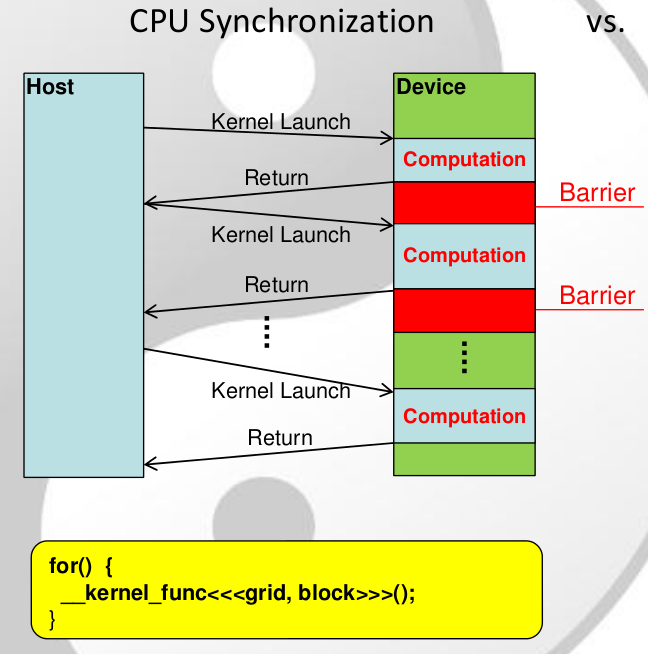
\includegraphics[width=100mm, keepaspectratio]{figures/Implicit synchronization.png}
	\caption{A kooperatív csoportok megjelenése előtt az egyetlen járható út teljes GPU szinkronizálásra. Látható, hogy gyakorlatilag minden programozási alapelvnek ellentmond. \textcolor{red}{UTALÁS}}
	\label{fig:Implicitsync}
\end{figure}

%TODO UTALÁS

A módszer több szempontból problémás. Egyrészt egy kernel hívása sok erőforrást igényel, ezért lehet, hogy sok kernelhívás mellett lassabb lesz a program, mintha egy szálon CPU-n futtattuk volna. Másrészt ha az eredeti függvényben ciklus iterációnként akarnánk szinkronizálni, akkor Implicit szinkronizációs módszer mellett a kernelhívásokat kéne CPU cikluson belülre helyezni. Ez még jobb esetben átláthatatlan és fenntarthatatlan kódot eredményez, de rosszabb esetben a grafikus kártya meghibásodását is okozhatja a sűrű kernelhívás miatt. A probléma tehát adott, de nézzük, hogy a kooperatív csoportok hogyan jelentenek erre megoldást.

Ahhoz, hogy grid csoporton belül szinkronizáljunk, első ránézésre elég a \textit{grid.sync()} függvényt használnunk, mint ahogy azt a thread blokkon belül is tettük.

\begin{lstlisting}[style=CStyle]
	grid_group grid = this_grid();
	grid.sync();
\end{lstlisting}

A főbb különbséget ott tapasztaljuk, amikor a kernel hívására kerül sor. A szokásos < < <...> > > konfigurációs szintaktika helyett a CUDA runtime API hívást kell végrehajtani (vagy annak driver megfelelőjét) \cite{CooperativeLaunchkernel}

Többféle módszer van a megfelelő több blokkos API hívásra, ezek közül nézzünk párat.
Ahhoz, hogy biztosítsuk a thread blokkok megfelelő együttműködését a GPU-n, a blokkok száma előre megfontolandó. Ahhoz, hogy annyi blokkot futtassunk, ahány Streaming Multiprocessor (SM) van beépítve a rendszerbe, az alábbi kód alkalmas:
\begin{lstlisting}[style=CStyle]
	int device = 0;
	cudaDeviceProp deviceProp;
	cudaGetDeviceProperties(&deviceProp, device);
	// initialize, then launch
	cudaLaunchCooperativeKernel((void*)my_kernel, deviceProp.multiProcessorCount,numThreads,args);
\end{lstlisting}

Ajánlott megvizsgálnunk, hogy a kernel hívásához mekkora maximális blokkPerSM aránnyal dolgozhatunk (legfeljebb hány blokk fér el egy SM-en). Tegyük, fel, hogy szükségünk van 128 szálra, akkor így járhatunk el. A CUDA documentation az alábbi példakódhoz hasonló eljárást javasol:

\begin{lstlisting}[style=CStyle]
	/// This will launch a grid that can maximally fill the GPU, on the default stream with kernel arguments
	int numBlocksPerSm = 0;
	// Number of threads my_kernel will be launched with
	int numThreads = 128;
	cudaDeviceProp deviceProp;
	cudaGetDeviceProperties(&deviceProp, dev);
	cudaOccupancyMaxActiveBlocksPerMultiprocessor(&numBlocksPerSm, my_kernel, numThreads, 0);
	// launch
	void *kernelArgs[] = { /* add kernel args */ };
	dim3 dimBlock(numThreads, 1, 1);
	dim3 dimGrid(deviceProp.multiProcessorCount*numBlocksPerSm, 1, 1);
	cudaLaunchCooperativeKernel((void*)my_kernel, dimGrid, dimBlock, kernelArgs);
\end{lstlisting}

Érdemes futtatás előtt ellenőrizni, hogy grafikus kártyánk egyáltalán támogatja-e a grid szinkronizációt. Ennek komoly feltételei vannak:
\begin{itemize}
	\item Csak 6.0 compute capability eszközök támogatottak
	\item Támogatott Windows operációs rendszer - Aktuális verziók: 8.1/10/11 \cite{supportedWinOS} 
	\item MPS ellátott Linux rendszer esetén csak 7.0 compute capability eszközök támogatottak
\end{itemize}


Az alábbi kód a cudaDevAttrCooperativeLaunch eszköz attribútumot vizsgálja meg.
\begin{lstlisting}[style=CStyle]
	int dev = 0;
	int supportsCoopLaunch = 0;
	cudaDeviceGetAttribute(&supportsCoopLaunch, cudaDevAttrCooperativeLaunch, dev);
\end{lstlisting}

Ez 1-be állítja a supportsCoopLaunch flaget ha a művelet támogatott a 0-s eszközön (egy grafikus kártyás rendszeren ez az alapértelmezett eszköz).

\subsubsection{Program felkészítése több blokkos futtatásra}
Mint azt már tárgyaltuk, bizonyos thread szám felett (jelenlegi GPU-kon 1024) a kerneleket már több blokkon szükséges futtani hardveres okokból kifolyólag. Amennyiben elég egy blokk használata, márpedig számos alkalommal ez a helyzet, ki tudunk használni olyan trükköket gyorsításra, mint például a \href{https://docs.nvidia.com/cuda/cuda-c-programming-guide/index.html#shared-memory}{gyors megosztott memória} használata a globális device memória helyett vagy a warpok hatékonyabb kihasználása. Előnyös lehet, ha algoritmusunkat egy és több blokkos használatra is megírjuk. Így képesek leszünk kezelni nagy thread számokat is, míg kis thread szám esetén kihasználjuk a lehetséges optimalizálási tulajdonságokat.



\subsection{CUDA használata Visual Studio alatt}

Szeretnék röviden leírást nyújtani az első CUDA nyelven megírt program létrehozásához.

\paragraph{CUDA Extension letöltése}
A gyártó bővítményt adott ki, mely a Visual Studio nevű fejlesztői környezetbe importálható. A CUDA legfrissebb verziója \href{https://developer.nvidia.com/cuda-downloads}{[az alábbi webhelyen]} tölthető le (A link később változhat). Itt lehet tájékozódni a program használati feltételeiről is. Főbb információk: néhány (3-4) GB tárhelyre, illetve 64 bites Linux vagy Windows operációs rendszerre van szükség.

\begin{figure}[ht!]
	\centering
	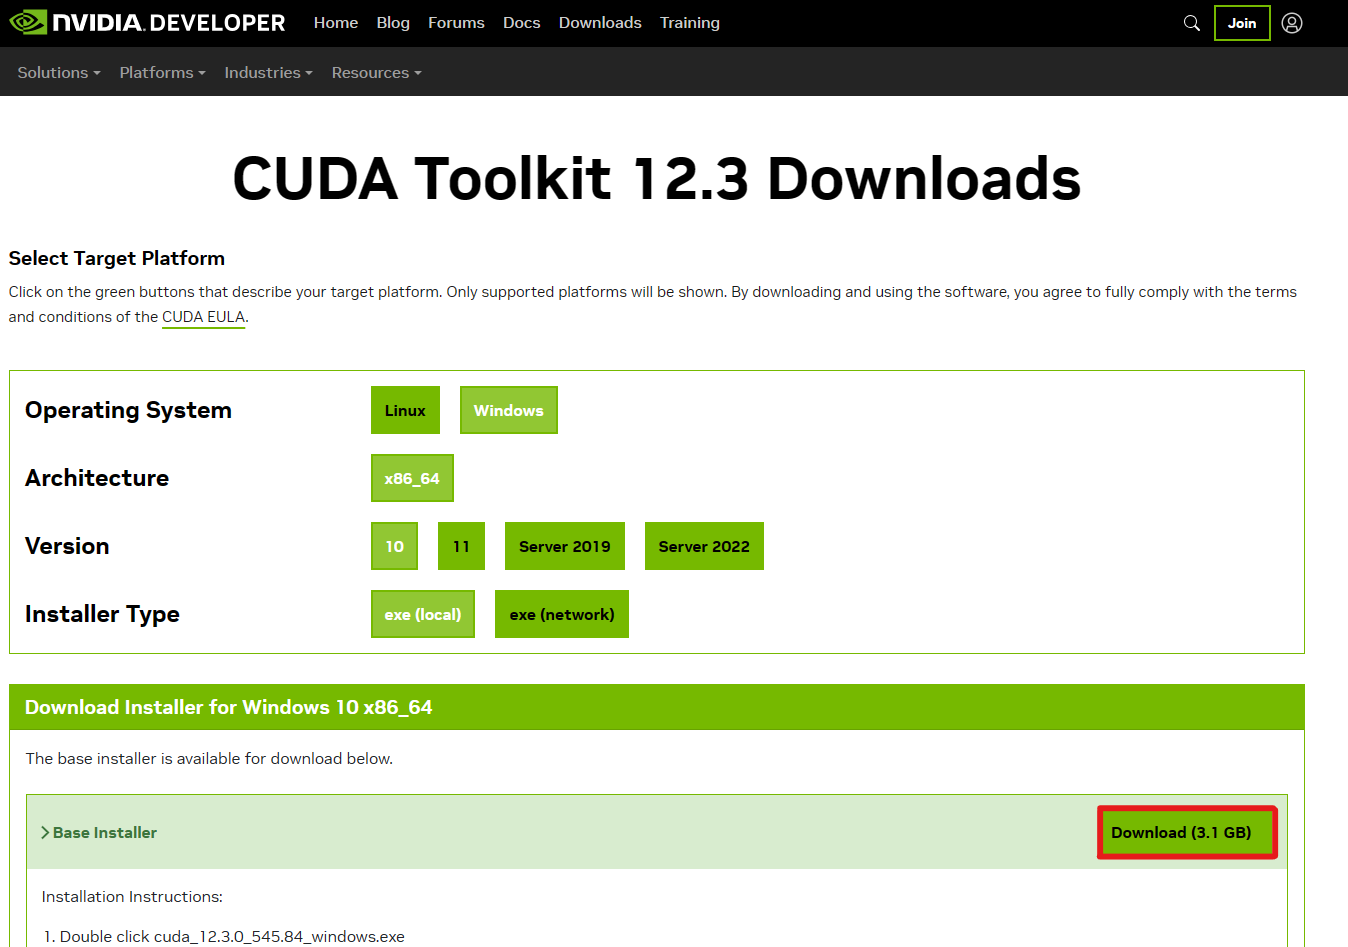
\includegraphics[width=150mm, keepaspectratio] {figures/install-1.png}
	\caption{1. lépés: A CUDA letöltése}
\end{figure}

\paragraph{Új projekt létrehozása}
Telepítés után ha új projekt létrehozását választjuk (File/New/Project), akkor "CUDA [verziószám] Runtime" néven kiválasztható a projekt típusának a CUDA. Adjunk neki egy nevet és egy elérési mappát, és létre is jön a projektünk.

\begin{figure}[ht!]
	\centering
	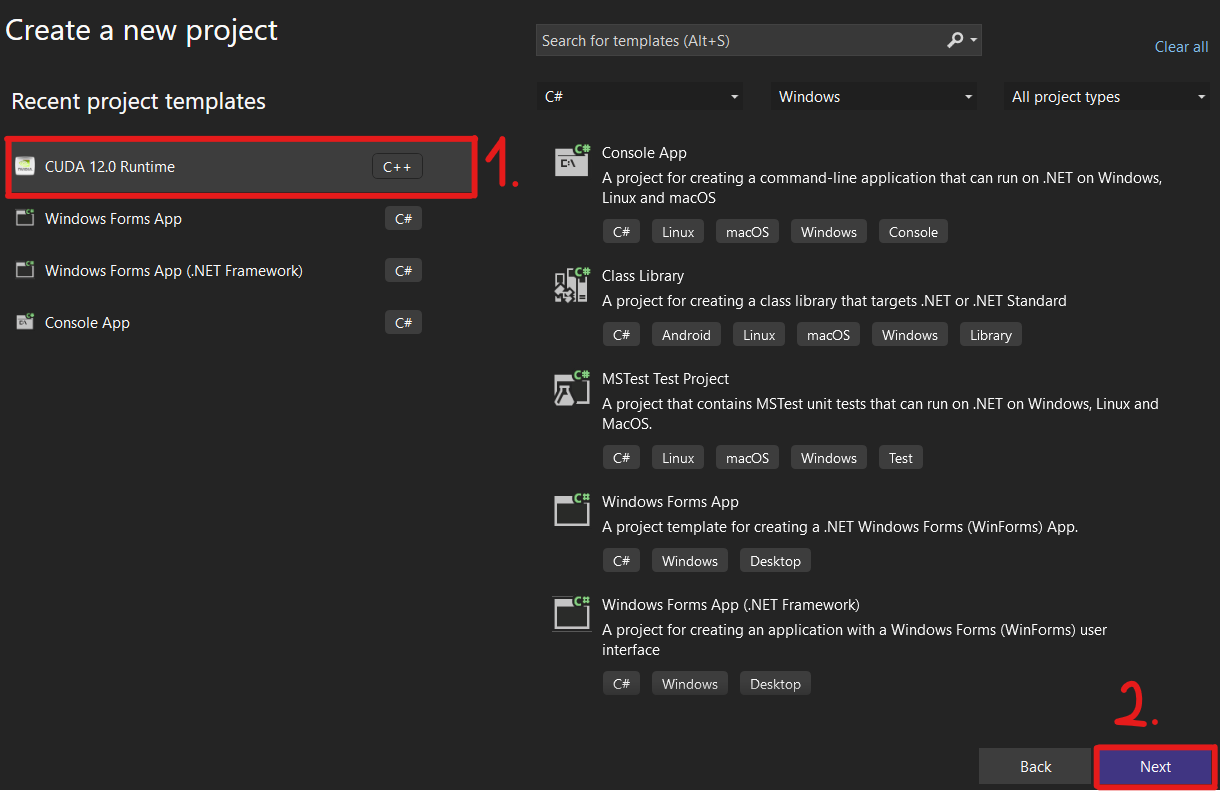
\includegraphics[width=150mm, keepaspectratio] {figures/install-2.png}
	\caption{2. lépés: Új CUDA projekt létrehozása}
\end{figure}

\paragraph{Példakód futtatása}
A template egy példaprogramot tartalmaz, amely két vektor összeadását végzi el videokártyán.

A kernel függvény nagyon egyszerű, mindössze 2 sorból áll: \cite{CUDAdoc}
\begin{lstlisting}[style=CStyle]
	__global__ void addKernel(int *c, const int *a, const int *b)
	{
		int i = threadIdx.x;
		c[i] = a[i] + b[i];
	}
\end{lstlisting} 

A "Local Windows Debugger gomb" megnyomásával lefut a kód, és meg is kapjuk az eredményt. Ezután már írhatunk saját kódot is.

\begin{figure}[ht!]
	\centering
	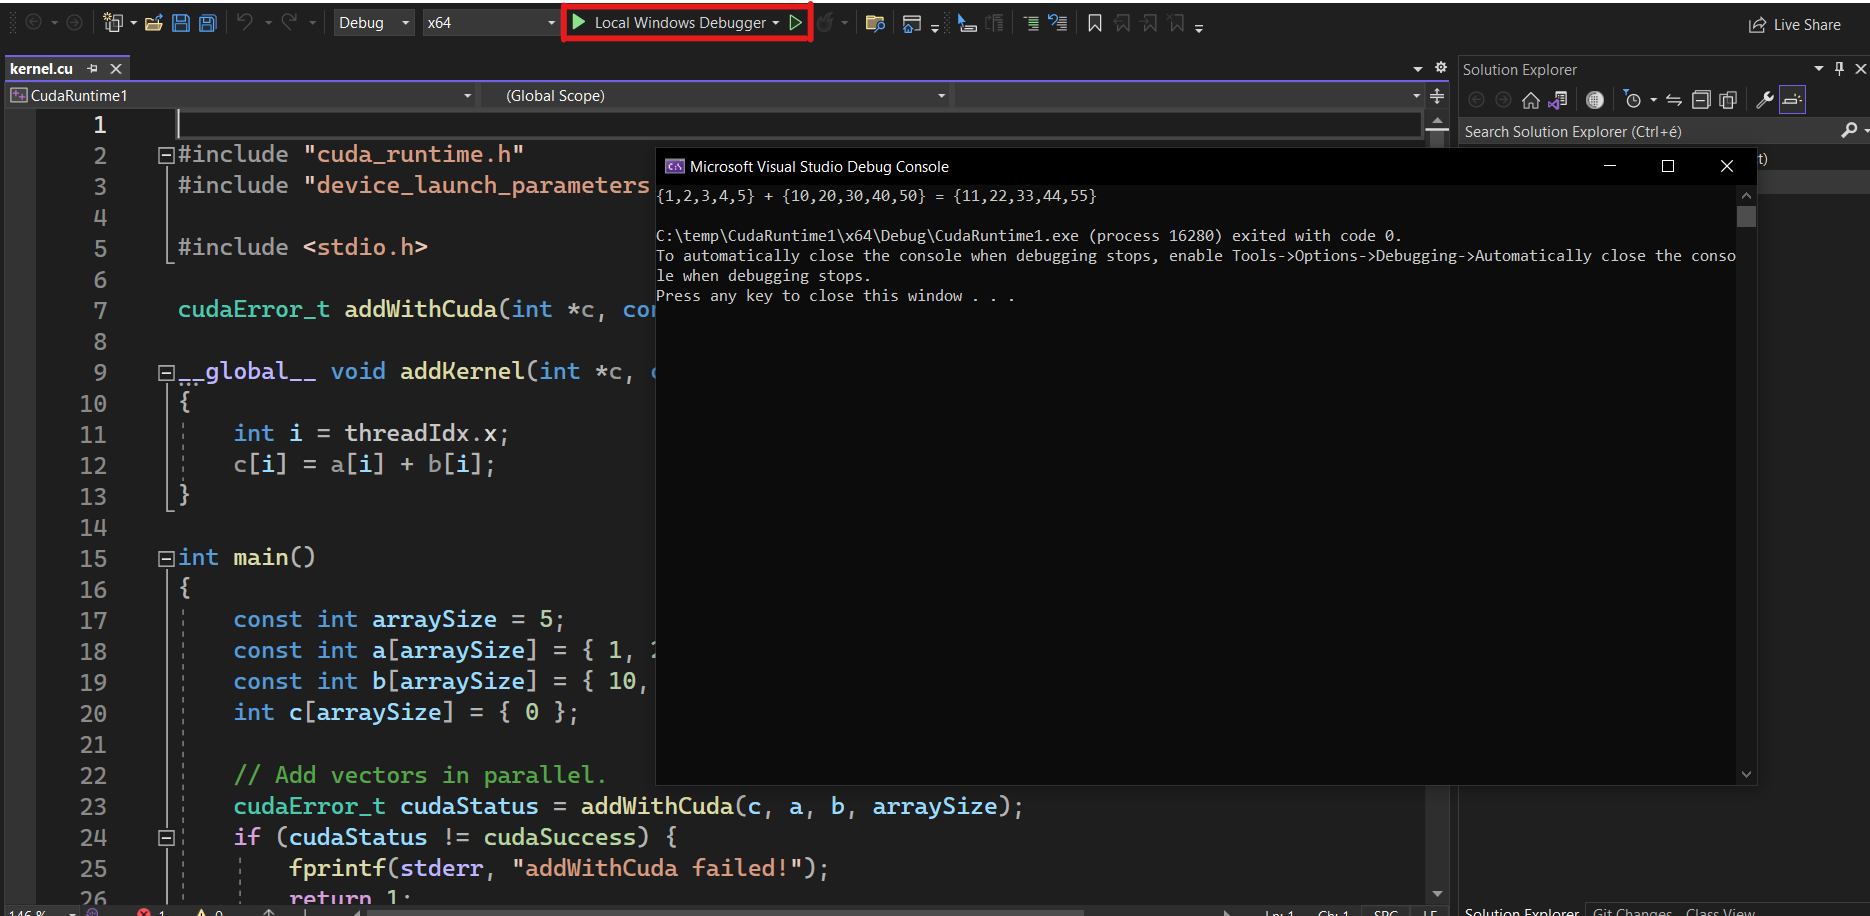
\includegraphics[width=150mm, keepaspectratio] {figures/install-3.png}
	\caption{3. lépés: Példakód futtatása}
\end{figure}